%% Beispiel LaTeX-Kapitel f�r deutschsprachige Technik Monographien
%% kann �ber die Datei engig.tex kompiliert werden
%% mit CL2eMONO.sty

\chapter{Die photographische Kamera}

Der nachfolgende Text enth"alt keine neuen Hinweise zum Layout. Dieses Kapitel dient lediglich als Test f"ur die
beigef"ugte root-datei \index{root-datei} \lq engig.tex' und
entspricht daher dem vorangegangenen Kapitel. Weitere
Einzelheiten und Hinweise zum Layout finden Sie unter \cite{JL1}. Selbstverst"andlich hat
der nachfolgende Text keine wissenschaftliche Relevanz, sondern er dient lediglich als
praktisches
Beispiel f"ur die Layoutrichtlinien \cite{JL1} in Springer
Technikb"uchern.

\section{Gleichungen}
F"ur das Layout der folgenden Gleichung wurde der Eingabebefehl
\verb|\vec| und der in der Pr"aambel der
root-datei \glq engig.tex\grq\, definierten Eingabebefehl \verb|\umu|
verwendet.

\begin{equation}
\vec{x}=\mu y = 50\ts \umu {\rm m}\ts  .
\end{equation}

\subsection{Mehrteilige Gleichungen}
Wie Sie in obigem Beispiel sehen k"onnen, werden Gleichungen automatisch kapitelweise
numeriert, wenn Sie sie mit der
Syntax \verb|\begin{equation}| einleiten (das funktioniert jedoch nicht mit der
Syntax \verb|$...$|). Nachfolgend ein
Beispiel f"ur die automatische Teilnumerierung von mehrteiligen Gleichungen,
die mit Hilfe des Styles \verb|subeqnary.sty|
generiert wurden:

\begin{subeqnarray}
a & = & c + d \ts , \label{f2a}\\
e & = & f - d \ts  .\label{f2b}
\end{subeqnarray}

Um im Haupttext auf einzelne Untergleichungen verweisen zu k"onnen, verwenden Sie
bei der Zitierung im Text die Labels
der betreffenden Teilgleichungen, die dann beim TeX-Lauf entsprechend "ubersetzt
werden, z.B. in (\ref{f2a}) und
(\ref{f2b}).

\subsubsection*{Unterdr"uckung der Teilnumerierung.}
Wenn Sie die automatische Teilnumerierung bei einer mehrteiligen Gleichung unterdr"ucken m"ochten, benutzen Sie bitte
die Original-LaTex-Umgebung \verb|eqnarray| und schreiben Sie ans Ende der betreffenden Gleichung \verb|\nonumber|
und setzen Sie den Z"ahler auf~0:

\begin{eqnarray}
a & = & c + d \ts , \nonumber \\
e & = & f - d \ts .
\setcounter{eqsubcnt}{0}
\end{eqnarray}

\section{Abbildungen}

Sollten Ihre Abbildungen in elektronischer Form vorliegen, so bietet
es sich an, diese im eps-Format mit Hilfe des graphicx-Pakets direkt in
den Text einzubinden (s. nachfolgendes Beispiel in Abb.~\ref{eps2})

\begin{figure}
\sidecaption
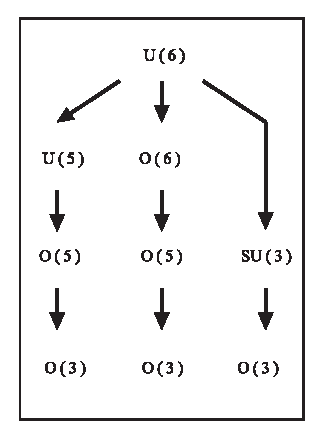
\includegraphics[width=.4\textwidth]{engifig.eps}
\caption[]{Beispiel einer elektronisch ein\-ge\-bun\-denen
eps-Abbildung}
\label{eps2}
\end{figure}

Als Platzhalter f"ur
Abbildungen, die nach\-tr"aglich montiert werden,
verwenden Sie bitte den Befehl
\verb|\mpicplace{Breite in cm}{H"ohe in cm}|.

Setzen Sie grunds"atzlich den Befehl \verb|\sidecaption| in der {\it
figure}-Umgebung. Falls gen"ugend Platz
($>$ 3\,cm) zur Verf"ugung steht, wird die Legende automatisch rechts neben die Abbildung gesetzt.

Aufbau und Layout des Legendeninhalts finden Sie beispielhaft in
Abb.~\ref{Teilabb2} und~\ref{Beschrift2} erl"autert.


\begin{figure}
\sidecaption
\mpicplace{9cm}{3cm}
\caption{Allgemeine Bildunterschrift. \ts({\bf a}) Die \glq
Bezeichnung\grq\, der Teilabbildung soll halbfett steil in
runde
Klammern gesetzt werden. ({\bf b}) Zur Erinnerung: Der letzte Satz einer Abbildungslegende
soll ohne Interpunktion
enden}
\label{Teilabb2}
\end{figure}

\begin{figure}
\sidecaption
\mpicplace{4cm}{5cm}
\caption{Diese Abbildung k"onnte unterschiedlich
formatierte Linien enthalten, um verschiedene Aspekte
eines Ph"a\-nomens darzustellen. Die Beschreibung dieser Linien sollte
zur leichteren Orientierung kursiv in runde Klammern gesetzt werden,
z.B. ({\it gestrichelte
Linie}). Grund\-s"atz\-lich soll der letzte Satz ({\it durchgezogene Linie}) ohne Interpunktion enden}
\label{Beschrift2}
\end{figure}

\section{Tabellen}

In den Springer Technikb"uchern erscheinen Tabellen (wie auch
Gleichungen und Abbildungen) und die dazugeh"origen "Uberschriften
{\it linksb"undig}. Wir empfehlen Ihnen,
"uberbreite
Tabellen m"oglichst auf Satzbreite zu bringen bzw. maximal 5\,mm "uber
den Satzspiegel hinausragen zu lassen.
Bitte verwenden Sie nachfolgende Tabellenbeispiele (Tabelle~\ref{Tab2a}
und ~\ref{Tab2b}) als Layoutbeispiel f"ur Ihre eigenen Tabellen.

\begin{table}
\caption[]{Kritische $N$ Werte}
\renewcommand{\arraystretch}{1.4}
\setlength\tabcolsep{5pt}
\begin{tabular}{llllll}
\hline\noalign{\smallskip}
${\mathrm M}_\odot$ & $\beta_{0}$ & $T_{\mathrm c6}$ & $\gamma$
  & $N_{\mathrm{crit}}^{\mathrm L}$
  & $N_{\mathrm{crit}}^{\mathrm{Te}}$\\
\noalign{\smallskip}
\hline
\noalign{\smallskip}
 30 & 0.82 & 38.4 & 35.7 & 154 & 320 \\
 60 & 0.67 & 42.1 & 34.7 & 138 & 340 \\
120 & 0.52 & 45.1 & 34.0 & 124 & 370 \\
\hline
\end{tabular}
\label{Tab2a}
\end{table}

\begin{table}
\caption[]{Brechungsindizes verschiedener optischer
Materialien. Tabellen"uberschriften bzw. Abbildungslegenden
werden automatisch linksb"undig gesetzt
}
\renewcommand{\arraystretch}{1.4}
\setlength\tabcolsep{14pt}
\begin{tabular}{@{}llll}
\hline\noalign{\smallskip}
Material & Brechungs- & Material & Brechungs- \\
& index $n$ && index $n$ \\
\noalign{\smallskip}
\hline
\noalign{\smallskip}
Luft & 1,0003 & Natriumchhlorid & 1,54 \\
Wasser & 1,33 & leichtes Flintglas & 1,57 \\
Magnesiumfluorid & 1,38 & schweres Flintglas & 1,66 \\
Kronglas & 1,52 & Titandioxid & 2,4--2,9 \\
\hline
\end{tabular}
\label{Tab2b}
\end{table}





\section{Listen}
Wir haben die {\it itemize}-Umgebung (labelitemi) dahingehend
ver"andert, da"s anstelle der Spiegelstriche jetzt Punkte vor den
einzelnen Aufz"ahlungspunkten erscheinen. Wir finden, da"s die Listen so

\begin{itemize}
\item
klarer erscheinen
\item
besser aussehen
\item
mehr ins Auge fallen
\end{itemize}

\section*{Zusammenfassung}
\addcontentsline{toc}{section}{Zusammenfassung}
\markright{Zusammenfassung}

Zusammengefa"st kann man sagen, da"s es eine ganze Reihe von Dingen zu
beachten gibt, bis ein Buchmanuskript tats"achlich zum Druck gehen
kann. Doch das sollte niemanden davon abhalten, ein Buch zu schreiben,
denn die Mitarbeiter des Springer-Verlags bieten den Autoren jede nur
m"ogliche Unterst"utzung an -- vorausgesetzt, da"s beide
Seiten fr"uhzeitig und offen miteinander kommunizieren.

\section*{"Ubungen}
\addcontentsline{toc}{section}{"Ubungen}
\markright{"Ubungen}

\subsubsection*{2.1} Wir w"urden uns freuen, wenn Sie sich f"ur die
Aufgaben an das vorgeschlagene Layout hielten -- die Aufgaben sollten
immer am Ende des betreffenden Kapitels stehen und eine unnumerierte
Abschnitts"uberschrift erhalten.

\subsubsection*{2.2} S"amtliche L"osungen sollten gesammelt am Ende des
Buchs -- noch vor dem Literaturverzeichnis -- stehen.

